\documentclass[10pt]{sigplanconf}
\usepackage{times}
\usepackage{datetime}
\usepackage{url}
\usepackage{hyperref}
\usepackage{amssymb}
\usepackage{amsmath}
\usepackage{todonotes}
\usepackage{graphicx}
\usepackage{subcaption}
\usepackage{multirow}
\usepackage{color,soul}

\conferenceinfo{SOSP'17}{October 29--31, 2017, Shanghai, China}
\copyrightyear{2017}

\newcounter{note}
 \newcommand{\note}[2][]{%
    % initials of the author (optional) + note in the margin
    \refstepcounter{note}%
    {%
        % \setstretch{0.7}% spacing
        \todo[color={red!100!green!33},size=\small]{%
            \textbf{Comment [\uppercase{#1}\thenote]:}~#2}%
}}

% These only appear when the 'preprint' option is specified.
% Enabling these will cause the first page of the document to fail the
% format check on HotCRP :-(

\titlebanner{Under submission to SOSP 2017 - do not cite or distribute}
\preprintfooter{Draft of {\currenttime}, \today{}}

% Paper number and no. of pages as author
% TODO: Replace 'XX' with your paper number (assigned when you register abstract)
% TODO: Replace 'NN' with actual number of pages.
\authorinfo{Paper \textbf{\#175}}{NN pages}

% No date in title area.
\date{}


\newcommand{\mech}{ARS}
\newcommand{\mechfull}{Application Resource Scheduler}

\begin{document}

\title{The Case for Cooperative Resource Sharing for Parallel Applications on Manycore Processors}
\maketitle

\section*{To fix/add}
\begin{itemize}
    \item 256 threads in experiments (over-provisioned)
    \item Why does contention happen?
    \item Scheduling algorithm details
    \item Other scheduling algorithms
    \item Expand related work
    \item Fix references
    \item How to modify parallelism in applications?
    \item Open source? How would we make this usable?
    \item Back-off punishment (i.e., delta between where you are and new rec -> amount of time to change)
    \item Compare with cooperative scheduling (i.e., yields)
    \item Expand beyond just CPU-intensive?
    \item Isolation vs virtualization
    \begin{itemize}
      \item OS can still take over
      \item Applications are responsible for changing behavior
      \item Other applications are not hurt if you don't change behavior (punishment)
    \end{itemize}
\end{itemize}

\begin{abstract}
The continuous rise of parallel and cloud computing has created new challenges for the systems community. On one hand, high-performance parallelized software requires close collaboration with the operating system and knowledge of underlying hardware. On the other, cloud computing environments attempt to provide an abstraction of a single-tenant system, typically by hiding those same details. This tension will get worse over time as application developers are pressured by the increasing number of cores available in server hardware.

Thus far, the systems community has prioritized maintaining the single-tenancy abstraction at the expense of global application performance. Server virtualization technologies like containers and virtual machines have become popular ways of maintaining isolation between applications that share hardware, but provide little means for cooperative resource sharing between applications.

In this world, developers seeking to maximize performance of their applications have two bad choices: either over-provision units of execution and run the risk of un-managed resource contention or under-provision them and fall short of performance potential.

We propose \mechfull{}s (\mech{}s), a mechanism for structured communication between the operating system and user-level applications for the purposes of cooperative resource sharing. \mech{}s allows applications to dynamically alter their behavior in response to changing resource availability, maximizing global and local application performance. We evaluate the feasibility of \mech{}s by using one to coordinate CPU usage across parallel execution of applications in the PARSEC benchmark, improving system throughput by up to 60\%.

\end{abstract}

\section{Introduction}

In recent years, economic and physical realities have pushed chip designers, application developers, and system administrators to rely increasingly on parallelism to satisfy performance demands~\cite{mack2011fifty}. 

Historically, the simplest way to increase application performance was to increase the clock speed of the running CPU. In general, increases in clock speed were driven by shrinking the die on the chip. However, the industry has reached the limits of this strategy: issues such as excess heat dissipation and quantum tunnelling have slowed the pace of miniaturization \cite{kish2002end}.

As a result, the semiconductor industry has been turning to multiprocessing designs to deliver steady performance gains. For over a decade now, multi-core processors have been widely available, utilizing the increasing number of transistors on a chip without a concomitant increase the CPU clock rates.  As an example, Intel introduced its first dual-core processor in 2005~\cite{intel2005pentiumee}.  9 years later, Intel introduced a multiprocessor with 60 cores capable of running 240 threads in parallel~\cite{intel2013xeonphi3120a}.

However, parallel programs struggle to keep pace with the number of cores available, leading to a second trend: an increase in multi-tenancy in order to fully utilize processing hardware.

\subsection{Cloud computing and multi-tenancy}
Coincident with the the rise of hardware parallelism has been a shift to cloud-based computing. The availability of high-capacity networks, commodity hardware, and virtualization technologies made it attractive for many users to outsource their computing infrastructure to a specialized provider.

To achieve the economies of scale necessary to make cloud computing feasible, service providers commonly share hardware resources among many unrelated applications, while providing the illusion that each application is the sole user of its machine.

This illusion is maintained with the help of hardware and software virtualization. Technologies such as virtual machines and containers attempt to hide the multi-tenant nature of the system from users by further abstracting away details of the underlying hardware.

\subsection{Needs of high-performance parallelism and cloud computing environment are in tension}
Any resource allocation scheme for the cloud requires a delicate balance between application and service provider needs. 

Individual applications would like maximum performance for cost. In highly parallel applications, this requires intimate knowledge of the underlying hardware and operating system resources, as well as the guarantee that other actors will not interfere with them. 

Cloud providers would like to maximize resource sharing to keep hardware costs low. In addition, they would like high global throughput in order to increase the number of new users they can take on.

These desires are fundamentally at odds. Were each individual application to have its way, they would receive a dedicated server, increasing costs beyond what is feasible for the for the provider. Were the cloud provider to have their way, application performance would suffer greatly.

This has resulted in an uneasy truce between users and providers. Applications that are sensitive to noisy neighbors over-provision in order to reserve excess capacity, while cloud providers under-provision instances to backstop performance.

\subsection{Isolation abstraction limit application performance}
Maintaining the illusion of that each application is the sole user of a machine has served operating systems well. However, in a highly parallel, multi-tenant systems, this illusion can inhibit application performance.

Applications designed for high-performance parallelism are typically as "greedy" as possible, attempting to take full advantage of known hardware resources. When many such applications share the same hardware resources, contention for system resources increases, causing unnecessary overhead and causing both individual and total application throughput to suffer.

\subsection{The case for cooperative resource sharing}
For the most part, research on multi-tenancy in the cloud has borrowed heavily from earlier work on multiprogramming in operating systems~\cite{krebs2015performance}. Particular emphasis has been placed on suitable ways to preempt or throttle bad actors in the system to maintain the illusion of isolation~~\cite{multitenancy2012enforcing}. 

However, modern cloud environments do not have the same characteristics as general-purpose operating systems. Often, servers run many copies of the same application for different users, with the application code being under the full control of the server owner.

Moreover, highly parallel computing workloads often do not benefit from systematic ``hiding'' of underlying hardware characteristics. As discussed above, parallel programs seek make full use of existing cores, and often assume they have exclusive access to these resources.

In such an environment, there is opportunity for a cooperative resource sharing model to enable ``denser'' multi-tenancy without sacrificing application performance.

Cooperation over resources requires that the operating system communicate information about resource state to user-level applications, allowing cooperating applications to adjust their run-time behavior accordingly.

This paper presents \mechfull{}s as a mechanism to implement cooperative resource sharing for highly parallel applications. The \mech{} has the following components:
\begin{itemize}
    \item A \textbf{message bus} enabling structured communication between the operating system and user-level applications.
    \item A \textbf{scheduler} that allocates resources between different applications and passes messages to them through the communication channel.
    \item A \textbf{client library} that allowed applications responds to scheduler messages by adjusting runtime behavior.
\end{itemize}

\subsection{Contributions}
Based on these observations, we present the following contributions:
\begin{enumerate}
  \item Observing that current operating system abstractions do not handle contention gracefully when running multiple parallel applications on the same manycore processor and that a cooperative approach may be more suitable
  \item Making the case for a structured and dynamic communication mechanism between applications and the operating system to restrict parallel applications and adjust the operating system scheduler
  \item Demonstrating that a cooperative approach with the right mechanism can improve system throughput by up to 60\%.
\end{enumerate}

% \section{Current application-OS abstractions}

Modern operating systems give the illusion to applications that they have dedicated access to all resources. In a typical operating system, an application has a dedicated user address space with a set of system calls to access system resources and services. The operating system provides the hardware abstraction layer to virtualize all hardware so the application may assume it has complete control over the entire machine.

On the other side of the barrier, the operating system kernel is responsible for running applications and providing them with address spaces along with CPU and other hardware resources. The kernel treats applications as black boxes to isolate and manage.

\subsection{These abstractions are inadequate}
However, such abstractions encourage applications to assume full access when they do not truly know what hardware resources are available to them at a given time. In the case of parallel programming, the concept meant to clarify may actually obfuscate. As a simple example, developers will frequently structure their applications to provision as many threads as the hardware will allow.

Further inspection reveals that the abstraction barrier can be breached in many ways. Applications can use a variety of directives and system calls to learn about underlying resources and the operating system can monitor application behavior or receive hints via those same system calls. These mechanisms suggest via proof by existence that the abstraction barrier simply is not adequate in many use cases.

\subsection{Increasing core counts and co-tenancy will exacerbate the inadequacies}

As core counts increase, individual applications struggle to make efficient use of all available resources. The newest Intel boards sport nearly 300 general-purpose cores. As cluster managers and cloud providers migrate to these manycore chips, they become burdened with the economic need to saturate their hardware. Packing many applications onto a single node becomes a increasingly common reality. These trends strain the illusion that applications still have their exclusive access to hardware.






\begin{itemize}
  \item For example, the Linux scheduler treats applications almost as black boxes. Schedules threads independently (limited within a process e.g., where threads / processes are spawned may give some cache locality). Used to have some heuristics to determine interactivity, but CFS no longer includes~\cite{molnar2007cfs}. The traditional approach to improve the utilization for multi-core or many-core processors is to schedule ready threads to run available CPU cores [cite ...].  ...
  \item Some control with cgroups to coordinate groups of threads, but not perfect (e.g., if there are too many threads, the scheduler cannot schedule them all within a single epoch without going below the minimum time granularity, then the epoch will increase; still `fair', but cycle is longer).
  \item Further abstraction from hardware (e.g., containers/VMs): application gets illusion of some resources that may be far from reality; OS treats applications as black boxes
\end{itemize}

\subsection{Even today, the abstraction is inadequate}
Because we break it all the time. As evidenced by:
\begin{itemize}
\item Hardware can get information / specific instructions from applications re how to do its job via directives and other DSLs (e.g., \texttt{LIKELY}, \texttt{UNLIKELY}, \texttt{atomic})
\item OS can get hints from application via sys calls (e.g., setting processor affinity)
\item Applications can get information about resources via syscalls, hardware/software counters
\end{itemize}

\begin{itemize}
	\item Under-provisioning threads can lead to low resource utilization
    \item Over-provisioning can create contention for resources and the system may thrash
 	\item Over-provisioning may cause low utilization on many core (not in the sense of having idle CPUs, but in the sense of eating up more total CPU to complete the job than at lower level of parallelism; need to explain this clearly so people aren't confused by `low utiliation'). CPU share and quota (cgroup) not enough; need to change parallelism of applications to affect utilization (different overheads / slow-down in total CPU time). different applications have various speedup curves [cite splash, PARSEC], depending on the granularities of computational components, cache localities and synchronization overheads and so on.  Applications with relatively poor speedup curves do not scale well on a large number of CPU cores.  In other words, it does not utilize the parallel processing power.
\end{itemize}

\subsection{Attempting to infer information across the barrier implicitly is hard}
\begin{itemize}
\item OS inferring about application. History of Linux scheduler. O(1) scheduler tried to classify applications based on behavior. Got so complicated that scrapped in favor of CFS.
\item Application inferring about hardware. Can get hardware info or set affinity, but if not coordinated, can lead to thrashing / over-taxed resources. Can work well for single applications. \cite{reinders2007intel}\cite{hellerstein2008optimizing}
\end{itemize}
\subsection{Even if you could infer information, active cooperation is impossible}
Maybe put this into the above section
\textbf{SEGUE}: show one problem of applications fending for themselves
\subsection{Talk about how this fits into a cloud environment}
For example: now we have yet another barrier: container/VM. So we are multiplexing over multiplexing over the underlying hardware.

\section{Application isolation abstractions cause resource contention}
This section characterizes the performance of parallel applications under different levels of parallelism, paying particular attention to program behavior when parallelism is high. Based on this characterization, we argue that the exisiting isolation abstractions are inadequate for multi-tenant, highly parallel workloads.

While many classes of applications might benefit from cooperative resource sharing, this paper focuses its evaluation on highly parallel applications. We chose to focus on parallel applications because:
\begin{enumerate}
    \item Cloud computing workloads are commonly parallel. Due to trends in commodity hardware, parallellizing work will even more important in the future.
    \item Parallel workloads uniquely benefit from detailed knowledge of the underlying hardware. They would like to utilize all cores if possible, and often need to micro-optimize to maximize cache hits.
\end{enumerate}

When optimizing parallel programs, application developers must carefully balance the performance benefits of increased concurrency with the performance costs of interference between concurrent activities.

Therefore, deciding how much parallelism to introduce in a program is one of the most important decisions an application developer can make. While it is obvious why under-using parallelism sacrifices performance, the ``upper bound'' is less understood.

\begin{figure}[t!]
    \centering
    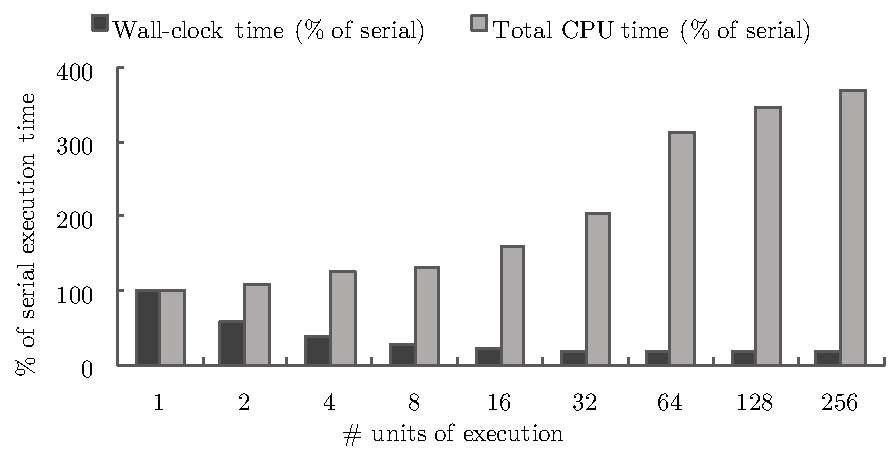
\includegraphics[width=8cm,height=4cm]{fig/speed-up.pdf}
    \caption{Wall-clock and total CPU execution times of the \texttt{bodytrack} application from the PARSEC benchmark suite~\cite{bienia2008parsec}. Increasing parallelism typically improves wall-clock execution time. However, total CPU time can increase, using more CPU resources to complete the same job. As an example, increasing from 16 to 32 threads increases total CPU time by approximately one-third, but we only see negligible improvement in wall-clock time.}
    \label{fig:speed-up}
\end{figure}

\subsection{Performance gains from parallelization are highly variable due to resource contention}
In a perfectly parallelizable workload, we would expect to see wall-clock execution speed up linearly with increasing parallelism. In real-world situations, however, wall-clock time typically speeds up sub-linearly with increasing parallelism (see Figure~\ref{fig:speed-up}).

\begin{figure}
\centering
  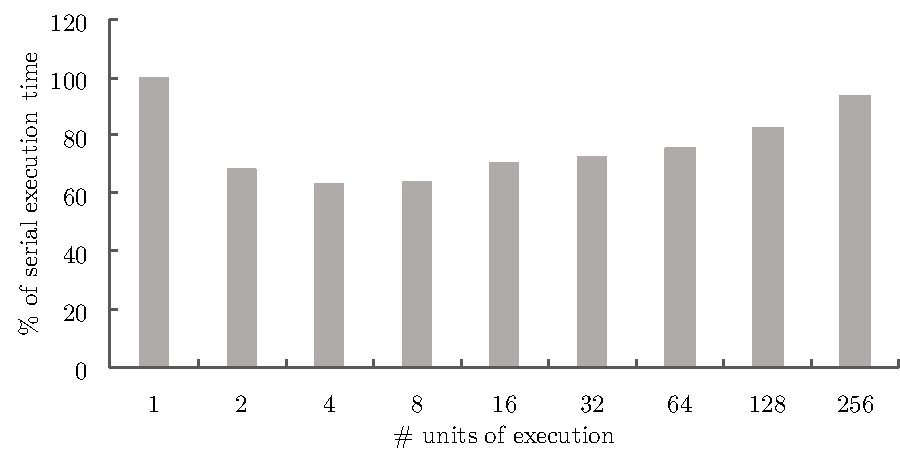
\includegraphics[width=8cm,height=4cm]{fig/contention.pdf}
  \caption{Wall-clock execution times for a job consisting of 16 instances of the PARSEC benchmark application \texttt{fluidanimate}. In each observation, we start the 16 instances simultaneously, all with the same number of threads (varied in along the x-axis). Parallel applications are designed to perform better with more units of execution, but performance can quickly degrade under contention.}
  \label{fig:contention-same}
\end{figure}

Clearly, increasing parallelism comes with costs. These costs are well documented, and include:
\begin{itemize}
  \item \textbf{Hardware resource contention.} CPU cores, main memory, bus throughput, etc. 
  \item \textbf{Context switch overhead.} Kernel time, cache invalidation, etc.
  \item \textbf{Synchronization overhead.} Common primitives (mutexes, semaphores, etc.) introduce overhead when contended for.
\end{itemize}

For most embarrassingly parallel problems, synchronization overhead is not high, as mutex contention is minimal. Context switch overhead can largely be reduced to a resource contention problem, as the cost of a context switch is dominated by cache invalidation~\cite{li2007quantifying}. Thus, we focus on the costs stemming from hardware resource contention.

\subsection{Isolation abstractions cannot solve resource contention}
We argue that the existing abstractions are inadequate for handling resource contention in multi-tenant, highly parallel workloads. The illusion of a single-user machine causes applications to systematically overuse finite hardware resources. As long as applications can expect to be ``greedy'' with regard to the hardware resource they are presented with, they will behave badly in multi-tenant environments (see Figure 2).

\subsubsection{Application doesn't know what resources it has}
In the existing scheme, user-level applications have the power to spawn threads and subprocesses, but little information about the state of hardware resources. Often, the degree of parallelism is statically determined by the application developer, with little regard for portability or the operating environment.

When the number of such applications on a given machine increases, the concurrent applications may not run efficiently. For example, on an Intel Xeon Phi processor with 64 cores, each supporting up to 4 hyperthreads, an application would create 256 threads for this hardware.  If its available hardware can only run a small number of threads because several applications are sharing the same machine, the overheads of 256 threads introduce inefficiency. 

% Figure  shows that the slowdowns of the PARSEC benchmark suite when using fewer number of CPU cores.  The worst case is XXX which slows down by a factor of 2 when running 256 threads on a single CPU core.

A common strategy to mitigate this problem to use a sophisticated dynamic parallelism library, such as Intel's TBB or Microsoft's TPL \cite{reinders2007intel}\cite{hellerstein2008optimizing}. However, this only performs optimization at the application level, running afoul of the scenario described above. Without understanding of the underlying resource environment, any application-local optimization cannot make globally optimal decisions.

\subsubsection{How applications are scheduled dramatically affects overall system performance}
The second reason is that the kernel does not have enough information to schedule multiple applications to maximize the efficiency or throughput of the hardware.  As an example, suppose an application has the following elapse times and speedups:
\begin{itemize}
\item
200 seconds on a single core.
\item 
12.5 seconds on 32 cores (16X speedup), with the best number of threads
for 32 cores
\item
10 seconds on 64 cores (20X speedup), with the best number of threads for 64 cores.
\end{itemize}

If the OS runs this application twice on the 64 core, one instance at a time, it will take 10 + 10 = 20 seconds.  However, if it runs two instances concurrently and each instance runs the best number of threads for 32 cores, it will take 12.5 seconds.  The throughput of the system improves by 37.5\%.

\subsection{Current trends in virtualization will exacerbate this issue}
Our arguments also apply to virtual machines and containers.  Virtual machine monitors provides virtualized hardware for an entire software stack including multiple operating systems.  Applications and their operating systems share the same abstractions as applications might on real hardware.

Containers provides isolated environments in a traditional operating systems rather than providing virtualized hardware. Within the context of a container environment, the abstractions between applications and their operating systems remain the same.

\begin{figure}[t!]
    \centering
    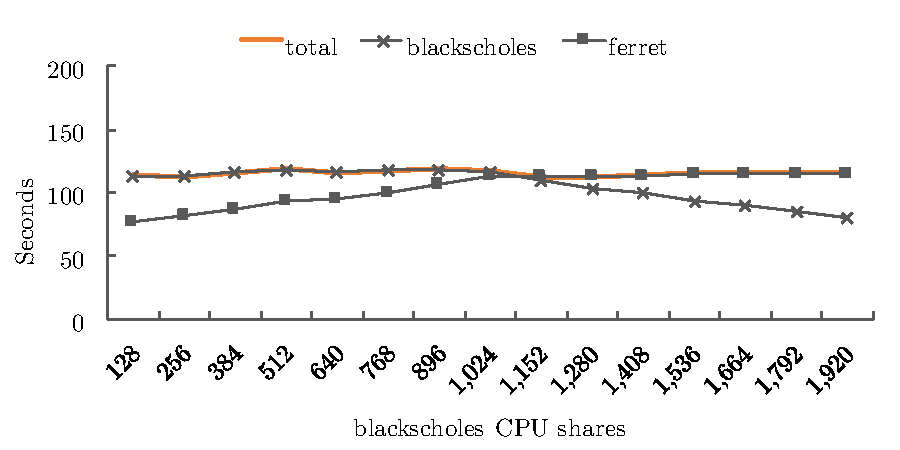
\includegraphics[width=8cm,height=4cm]{fig/without-application.pdf}
    \caption{Improving overall performance is difficult without true cooperation from applications.  In this simple example, we have a total of 2048 shares of CPU time that we divide among two applications, \texttt{blackscholes} and \texttt{ferret}, that start at the same time. We use Linux control groups to enforce that the two applications will have roughly the same ratio of time on CPU as the ratio of their weights. We can manipulate an application's resources with CPU shares, but we cannot alter application behavior via this mechanism and as a result, minimally impact the total execution time (orange, for those with color).}
    \label{fig:naive-cooperation}
\end{figure}
\section{The case for cooperative resource sharing}

\begin{figure*}[t!]
        \centering
        \includegraphics[width=16cm]{fig/\mech_diag.png}
        \caption{The design for a \mechfull{}, a proposed implementation of cooperative resource sharing}
        \label{fig:\mech{}}
\end{figure*}

Given challenges observed in the previous section, we advocate an extension to the traditional application-OS abstractions with a dynamic, bi-directional communication mechanism between applications and the OS scheduler, as shown in Figure 4. 

As long as applications are architected with the assumption that they have exclusive access to machine resources, resource contention is inevitable in parallel, multi-tenant environments. Developers will be required to over-provision compute capacity in order to avoid resource contention, and otherwise program and plan with the expectation that they are sharing a machine with others. They will not be fooled by the illusion that they the sole users of the system.

We argue for cooperative resource sharing as a preferable multi-tasking paradigm. In this scheme, applications are written with the full knowledge that they are co-tenants sharing resources, and agree to allow a centralized scheduler to control their resource consumption. We propose \mechfull{}s as a potential mechanism to implement cooperative resource sharing.

\subsection{Cooperative resource sharing may uniquely overcome resource contention problems}
When applications cooperate, they receive structured information about "real" system resources and instructions about how to utilize resources for greatest effect. In any system where isolation is a core guarantee, this information is by definition unavailable to the application.

Attempts to solve resource contention problems by strengthening isolation guarantees ultimately run up against this limitation. Slicing applications through virtualization does not change fundamental hardware facts (see Figure 3). 

\subsection{Modern cloud computing environments can limit the downsides of cooperation}
The fundamental flaw in cooperative multitasking schemes is that they rely on individual applications to behave themselves. A single bad actor in the system can monopolize resources, which creates a prisoner's dilemma where it is simpler for the scheduler to pre-empt tasks to ensure fairness.

However, in today's managed compute environments, all non-trivial applications running on a server are under the full control of the service's operator. For example, a multi-tenant database-as-a-service like Amazon's DynamoDB \cite{decandia2007dynamo} will consist of multiple tenants, all running proprietary Amazon code. In such an environment, ensuring that all applications "play by the rules" is simply a matter of integrating some mechanism like an \mech{} into the application code.

\subsection{What are scenarios under which we might use \mech{}s?}
In general, any environment that requires multitasking over several highly parallel applications could benefit from cooperative resource sharing. Some examples include:
\begin{itemize}
    \item \textbf{OLAP and batch processing workloads.} For big data analytics and data warehousing applications, many highly parallel jobs may be placed a single node. The application itself can be modified to cooperate with the \mech{}, and the interest of the service owner is likely to maximize global throughput per node.
    \item \textbf{Proprietary compute clouds.} Many companies operate private clouds, where all users and applications are under 
\end{itemize}

\section{Designing a CPU \mechfull{} for parallel programs}
This section discusses the design of a \mechfull{}, a system to enable cooperative resource sharing. This design is generalizable to any type of shared resource and any type of applciation, but in the interest of brevity we will discuss it in terms of sharing CPU resources between highly parallel applications.

\subsection{Message bus}
This component enables communication between the scheduler and client libraries hosted on each cooperating application.

It is important to note that, as a single component accessible to all applications, the message bus is itself a shared resource. Therefore, care must be taken that it does not become a bottleneck in the system.

To mitigate contention for this component, the scheduler and client libraries implement a stateful, asynchronous protocol over this message bus that allows them to operate independently of one another, decreasing the likelihood of synchronization overhead.
\subsection{Scheduler}
The scheduler is responsible for maintaining global resource state and allocating resource between cooperating applications in accordance with some predetermined policy.

In our example of a CPU-sharing \mech{}, the scheduler will decide how many software threads each application should be allowed.

\subsubsection{System poller}
To collect and store this information, the scheduler maintains a system poller that communicates with the operating system about hardware resources and stores the resulting data in a time-series data structure.

In the case of a CPU-sharing \mech, global resource state could, for example, consist of:
\begin{itemize}
    \item Number of cores and degree of hyperthreading
    \item Number of runnable processes
    \item Number of sleeping processes
\end{itemize}

\subsubsection{Application poller}
At the same time, the scheduler continuously checks for messages on the message bus. These messages provide confirmation that cooperating applications have indeed adjusted their behavior in accordance with the scheduler, as well as passing along any application-level data that the scheduling policy might require. 

Application-level data is likely to change over the life-time of application. This is especially true of applications with distinct phases of operation. Thus, it is sensible to store application-level data in a time-series data structure as well.

In the CPU-sharing case, the application would send the number of software threads it is operating with. Additional data shared could be, for example, application-specific performance instrumentation or user-specific SLAs.

\subsubsection{Scheduling policy}
Based on data gathered from the system poller and the application poller, the scheduler makes a decision on resource allocation to cooperating applications based on a its scheduling policy. These allocations are then communicated via the message bus to each application's client library.

The efficiency information of each application can be used by the policy achieve certain goals such as maximizing throughput, minimizing average latency, or maximizing hardware utilization. 

There is a wide body of operating systems research and industry work on the merits of various scheduling policies ~\cite{li2009scheduler}. We note that they could be implemented in any \mech{} scheduler.

\subsection{Client library}
The client library is hosted by all cooperating applications. In a typical cloud computing environment, all applications of non-trivial resource consumption will be cooperating, since the environment is under the full control of the system operator.
In the case of as CPU-sharing \mech{}, the client library has two modules:

\subsubsection{Message handler} 
This module periodically checks the message bus for any messages from the scheduler about how to adjust the application's resource consumption, and updates the client library's internal state accordingly. 

In the CPU-sharing case, the message from the scheduler takes the form of a recommendation for how many software threads to use.

\subsubsection{Resource controller}
This module takes the scheduler's recommendation about resource consumption and executes it by adjusting run-time application behavior. In the CPU-sharing case, this would take the form a thread pool which supports dynamic size adjustment. 

This is the module that is most tightly coupled with application logic. As a result, care must be taken to design the controller in a way that is easily integrated into existing systems. For example, the CPU-sharing resource controller could wrap a popular existing thread pool implementation, allowing clients to specify a starting size with the understanding that it may change over time. As another example, a memory-sharing resource controller could implement a dynamically-sized arena that applications use in place of ad-hoc memory allocation.

\section{Implementation considerations}
In this section, we discuss an example of a concrete implementation of a CPU-sharing \mechfull{} design. We begin by outlining some of our general design goals, and proceed by examining implementation considerations for each component.

\subsection{Design goals}
At a high level, we wanted our implementation to conform to the following goals:
\begin{itemize}
    \item \textbf{Low overhead.} As the primary purpose of cooperative resource sharing is to increase global application performance, care must be taken that our \mech{} implementation not become a practical bottleneck.
    \item \textbf{Graceful fallback.} To ease application integration, simplify testing, and increase robustness, our implementation should fall back to sensible default in the event that any component becomes unavailable.
\end{itemize}

In addition, we had the following non-goals:
\begin{itemize}
  \item \textbf{Exhaustive performance optimization.} Our goal was to make the case that cooperative resource sharing can improve performance for highly parallel workloads, not to tune a production environment for maximum efficiency.
  \item \textbf{Sophisticated scheduling policy.} Significant work has already been done in scheduling theory and practice. Our implementation need not retread existing ground to prove that cooperation is desirable.
  \item \textbf{Intrusive resource control.} While it may be tempting to specify elaborate resource acquisition and consumption requirements for applications, in practice this would require that developers substantially revise their computation models in order to integrate with our library.
\end{itemize}

\subsection{Message bus}
As a globally shared resource, message bus must be fast even in the presence of many clients. In practice, this means any implementation must achieve:
\begin{itemize}
    \item \textbf{Fast reads and writes.} An interprocess communication scheme must be chosen such that both the scheduler and client libraries have extremely fast access.
    \item \textbf{Low synchronization overhead.} Even with many (hundreds) of applications, there should be little or no contention for synchronization resources..
\end{itemize}

To achieve fast and reads and writes, we implement the message bus using shared memory as our communication medium. We create two channels in the allocated shared memory, corresponding to each direction of communication.

The scheduler-to-application channel contains messages regarding the scheduler's latest recommendation for the number of software threads for applications to use. The application-to-scheduler channel contains messages where applications register their existence with the scheduler and update their current thread count.

Both channels are protected by reader-writer locks to ensure that multiple readers do not contend for access to the channel. In our implementation, the client library only sends and receives messages every 500 milliseconds, which makes lock contention negligible in practice. If the latency of client response is a concern, finer-grained synchronization models are feasible (for example, giving each application it's own channel).

\subsection{Scheduler}
\subsubsection{Scheduling policy}
As sophisticated scheduling was a non-goal, we intentionally made our scheduler policy as minimal as possible. Our policy only requires one piece of system information to make allocation decisions: the number of runnable processes currently waiting to run. On this basis, a single recommendation is issued for all applications to follow. No distinctions are made between applications, and the scheduling policy only tries to maximize global application throughput.

\subsubsection{System poller}
For low overhead communication between the kernel and userspace, we rely on \texttt{procfs}. This allows the system poller to gather basic information about the system without the overhead of a system call or some dynamic tracing method. Our implementation only reads the \texttt{procs\_running} field of \texttt{/proc/stat}, which gives the number of threads currently running on CPU.

This information is gathered once per second and saved in a fixed-size time series data structure.

\subsubsection{Application poller} 
Our simple scheduling policy does not require information from the application. While we implemented a channel for the application to pass messages to the scheduler about the current number of threads it is using, this information is unused by the scheduler.

\subsection{Client library}
In implementing the client library, a decision needs to be made about when the resource controller will intervene to set the number of threads in the application. There are three options, each with varying levels of intrusion into the application logic:

\begin{enumerate}
  \item \textbf{Static parallelism.} This is equivalent to no resource controller at all; the number of threads is determined by user input.
  \item \textbf{Dynamic parallelism.} On start-up, the client library consults the scheduler for how many threads to use. This number is kept throughout the lifetime to the application.
  \item \textbf{Dynamic run-time parallelism.} Throughout the lifetime of the application, the client library continuously receives messages from the scheduler and resizes its thread pool accordingly.
\end{enumerate}

While dynamic run-time parallelism is the optimal resource control model from a performance perspective, it is highly intrusive and often requires the application developer to re-architect the concurrency model of their program. 

For example, the \texttt{canneal} benchmark in PARSEC uses a highly aggressive lock-free synchronization strategy that recovers from data races rather than try to avoid them~\cite{bienia2008parsec}. Changing the number of threads dynamically would require substantial effort, and repartitioning the work when changing thread count would require global locking that would sacrifice the performance benefits of a lock-free strategy.

Thus, while we implemented the features necessary for dynamic run-time parallelism in our client library, we opted to include a mode that disabled the run-time thread count updates. 

\section{Performance implications}
In our evaluations we seek to answer whether cooperative scheduling can meaningfully improve overall performance. Unless otherewise noted, we focus on overall system throughput. The workloads that might benefit most from our proposal--batch data analytics--motivate this choice.

\begin{figure*}
\centering
\begin{tabular}{|l|l|c|c|c|c|c|}
\hline
\multirow{2}{*}{\textbf{Name}} & \multirow{2}{*}{\textbf{Application domain}} & \multicolumn{2}{|c|}{\textbf{Parallelization}} & \multirow{2}{*}{\textbf{Working set}} & \multicolumn{2}{|c|}{\textbf{Data usage}} \\
& & \textbf{Model} & \textbf{Granularity} & & \textbf{Sharing} & \textbf{Exchange} \\
\hline
\textbf{\texttt{\text{*}blackscholes}} & Financial analysis & data-parallel & coarse & small & low & low \\
\hline
\textbf{\texttt{bodytrack}} & Computer vision & data-parallel & medium & medium & high & medium \\
\hline
\textbf{\texttt{\text{*}canneal}} & Engineering & unstructured & fine & unbounded & high & high \\
\hline
\textbf{\texttt{\text{*}dedup}} & Enterprise storage & pipeline & medium & unbounded & high & high \\
\hline
\textbf{\texttt{facesim}} & Animation & data-parallel & coarse & large & low & medium \\
\hline
\textbf{\texttt{ferret}} & Similarity search & pipeline & medium & unbounded & high & high \\
\hline
\textbf{\texttt{\text{*}fluidanimate}} & Animation & data-parallel & fine & large & low & medium \\
\hline
\textbf{\texttt{freqmine}} & Data mining & data-parallel & medium & unbounded & high & medium \\
\hline
\textbf{\texttt{\text{*}streamcluster}} & Data mining & data-parallel & medium & medium & low & medium \\
\hline
\textbf{\texttt{\text{*}swaptions}} & Financial analysis & data-parallel & coarse & medium & low & low \\
\hline
\textbf{\texttt{vips}} & Media processing & data-parallel & coarse & medium & low & medium \\
\hline
\textbf{\texttt{x264}} & Media processing & pipeline & coarse & medium & high & high \\
\hline
\end{tabular}
\label{table:parsec-apps}
\captionof{table}{Applications annotated with a * have been integrated with the \mech{} client library. This is a qualitative summary of all the workloads in the PARSEC benchmark. PARSEC workloads were chosen to cover different application domains, parallel models and runtime behaviors.~\cite{bienia2012characteristics}}
\end{figure*}
\subsection{Prototype implementation}
When implementing our prototype, we opted for simpler designs and heuristics. The message bus, scheduler, and client library together comprise fewer than 2000 lines of C and C++. Thanks to the design of the PARSEC benchmark suite, we were able to integrate the client library into many of the benchmark applications with fewer than 100 lines of modified code. To simplify communication among components, we use shared memory and locks, allowing us to forgo message queues or additional threads to maintain communication.

Although we implemented more complex mechanisms, we were able to demonstrate strong results using the most basic configuration. In the following experiments, the scheduler only polls the system-wide run queue and ignores any other system or application-specific data. Given that the target workloads are CPU-intensive, using thread contention as a proxy for resource contention is reasonable. Despite this simplicity, however, the application implicitly gives the scheduler a lot of information by registering as a client. Most importantly, the application signals that it is capable of dynamic run-time parallelism and is willing to follow directives from the scheduler.

During run-time, the scheduler provides applications with a recommended number of threads to create on start. We assume that applications are well-behaved, but it would not be difficult to implement punitive measures.

\subsection{Experimental environment}
We conducted experiments on four different machine types: a quad-core desktop (8 hardware threads), a dual-socket 9-core c4.8xlarge Amazon EC2 instance (36 vCPUs), a 4-socket 10-core workstation (80 hardware threads), and a cluster with many 68-core machines (272 hardware threads). Although our findings are consistent across machines, we choose to present results from the 68-core machines to illustrate the challenges introduced by these manycore chips.

The cluster is part of a research installation generously maintained by the Intel$^{\tiny{\textregistered}}$ Corporation and features 256 nodes each equipped with an Intel Xeon Phi\texttrademark CPU (Model 7250). Each Xeon Phi\texttrademark has 68 physical 1.4GHz cores with 4 hardware threads per core. Each physical core has 32K of L1d and L1i cache and shares a 1024K L2 cache with one other core. The CPU can be configured in several ways. First, we use the fully symmetric NUMA topology as opposed to the quadrant mode to simplify the profiling and debugging process. Second, we use the 16GB on-package memory as a large last-level cache rather than use it as ultra-fast memory so our results are more generally applicable to less sophisticated hardware.

\subsection{Benchmark applications}
To evaluate our \mech{}, we use a popular parallel application suite, PARSEC~\cite{bienia2008parsec}, to generate a large number of diverse workloads spanning several classes of parallel programs and problem domains (see Table 1). After integrating the client library into each application, we control their levels of parallelism as they enter the system. For six applications (see starred applications in Tabl 1), we also instrumented the capabiltiy to dynamically adjust parallelism during program execution. However, in experiments, we found that the overhead of such a design is only justified for longer-running applications residing with unpredictably busy neighbors.

\subsection{Baseline comparisons}
In order to create an apples-to-apples comparison unencumbered by differences in implementation, we chose to evaluate the workloads using two existing thread libraries with and without cooperation. We use the Pthreads standard as an example of lower-level parallel programming and the Intel$^{\tiny{\textregistered}}$ Thread Building Blocks (TBB) library as an example of a sophisticated industrial-grade library. Eleven of the twelve PARSEC benchmark applications are implemented using Pthreads and five also have TBB implementations.

\subsection{Generating workloads}
In order to compare performance, we create several hundred randomly-generated workloads by drawing samples from the set of benchmark applications. We focus our attention on constant load scenarios as these are most advantageous to the existing parallel programming libraries. More dynamic loads are amenable to our approach since they offer many opportunities to change an application's parallelism to adjust to new circumstances.

We run each workload with Pthreads and TBB in their normal use case and as part of a cooperative environment. For each of these four cases, we run for several levels of cotenancy, modeled by some constant number of simultaneously running applications.

\subsection{Coordinating with \mech{}s}
\begin{figure*}[t!]
    \centering
    \begin{subfigure}[t]{0.5\textwidth}
        \centering
        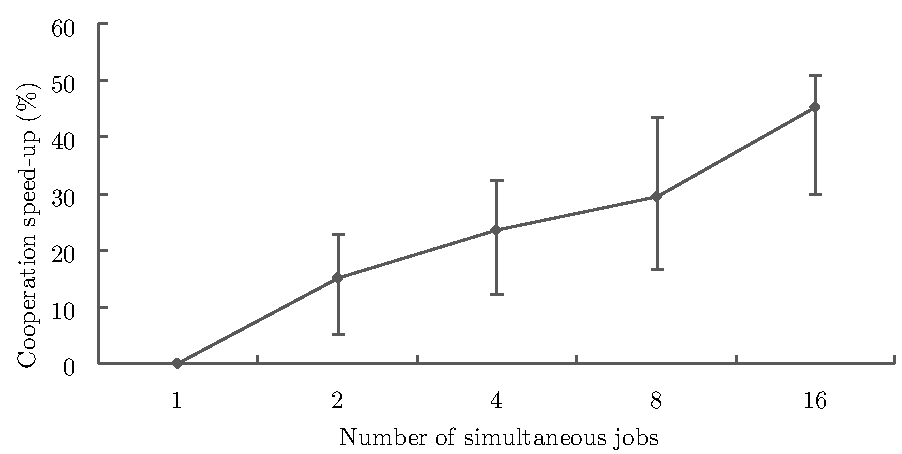
\includegraphics[width=8cm,height=4cm]{fig/randomized-pthreads.pdf}
        \caption{Pthreads implementation}
        \label{fig:pthread}
    \end{subfigure}%
    ~ 
    \begin{subfigure}[t]{0.5\textwidth}
        \centering
        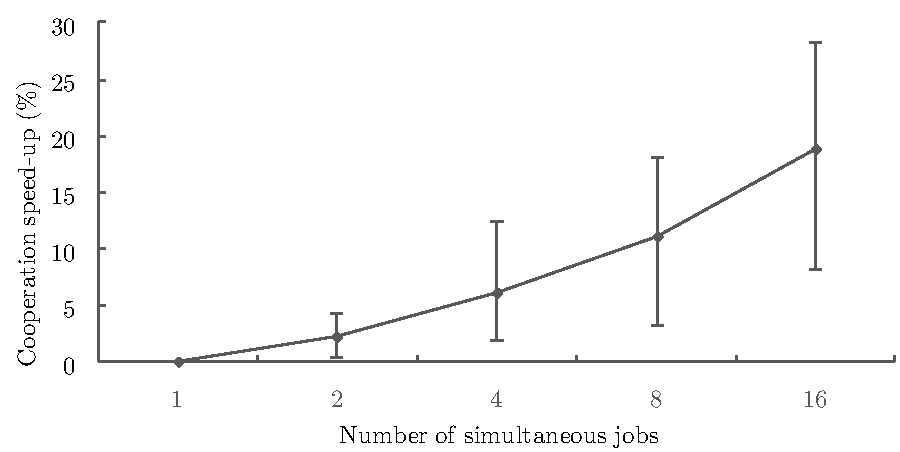
\includegraphics[width=8cm,height=4cm]{fig/randomized-tbb.pdf}
        \caption{Intel$^{\mbox{\tiny\textregistered}}$ Threading Building Blocks (TBB) implementation}
        \label{fig:tbb}
    \end{subfigure}
    \label{fig:randomized}
    \caption{The benefit from cooperation increases with contention. Each observation is 100 jobs (100 tasks each) run both with and without cooperation. The line represents the mean throughput (time to job completion) while error bars represent the maximum and minimum speed-ups we observed. Of note, we did not observe our mechanism harming performance.}
\end{figure*}
We show our main results in Figure 5. The pair of figures show the same experiments for Pthreads and TBB. The vertical axis indicates how much faster the cooperative approach completed workloads relative to the pre-emptive approach on the same workload. The line shows mean speed-up for the specified load level and the error bars show the maximum and minimum observed speed-ups.

There are two important observations. First, we did not observe in any scenario where cooperating led to a worse outcome. Second, cooperation improves performance to a greater extent with increasing contention. We were able to achieve such a result with a simple design because our workload has a number of structural features (e.g., CPU-intensive, parallel structure) that lend themselves to cooperation.

% \subsection{Characterizing results}



% We want to discuss the following and map to real-world workloads
% \begin{itemize}
% \item What we are good for: large-scale batch compute for big data. Individual latency doesn't matter; about throughput. Make sure to address the fact that analytics framework (e.g., spark) do parallelization at task / process level
% \item What we don't really affect
% \item What we are bad for
% \end{itemize}

% \subsection{Measure overhead}
% Don't compare against original implementation since that's apples and oranges. But here it is anyway for overhead purposes.

\section{Discussion and related work}
There are three broad areas of related work. First, there is a long and significant history of coordinating resources among applications. Second, there are several parallel programming libraries that touch on many similar ideas (e.g., monitoring resources, manipulating application behavior). Finally, from a broader perspective, there are the works that investigate and tease the application-OS interface.

\subsection{Coordinating resource consumption}
Coordinating resources is an important problem in many domains. In distributed systems alone, we have seen numerous takes on the problem \cite{yoo2003slurm}\cite{bhattacharya2013hierarchical}\cite{regehr2001using}\cite{chowdhury2014efficient}\cite{waterman2012coordinated}\cite{hindman2011mesos}\cite{ghodsi2011dominant}\cite{henderson1995job}. We acknowledge that we could not possibly mention all relevant approaches. Instead, we select a few diverse examples that specifically address a single node. We classify these approaches approximately as application-aware and hardware-aware.

Application-aware approaches have typically relied on application directives (e.g., \texttt{UNLIKELY}, processor affinity, DSLs like OpenCL), online monitoring, offline profiling, or some combination of the three. Gang scheduling~\cite{ousterhout1982scheduling} marks one of the earlier approaches to coordination, describing a mechanism for communicating units of execution to align and avoid blocking. Cache-~\cite{philbin1996thread} and contention-aware~\cite{blagodurov2010contention} schedulers examine historical application behavior to make intelligent resource allocations. Finally, the rich literature of real-time systems~\cite{liu1973scheduling}\cite{goyal1996hierarchical} demand very precise information from applications.

However, we observe that while these approaches make use of application information, they make decisions without the cooperation of applications. We believe that cooperative multitasking is most similar in spirit to our approach, but as evidenced by virtually all operating systems, it may have chosen dangerous abstractions.

% Unorganized
% \begin{itemize}
% \item \href{http://ethesis.inp-toulouse.fr/archive/00002747/01/tran.pdf}{resizing vms}: use VM's facilities to communicate new hardware reality to applications
% \item \href{https://www.usenix.org/legacy/events/osdi99/full_papers/banga/banga.pdf}{resource containers}
% \end{itemize}

By contrast, hardware-aware approaches attempt to probe information about underlying hardware~\cite{blagodurov2010case} \cite{topcuoglu2002performance} to make resource decisions. Perhaps most famously the Linux scheduler~\cite{molnar2007cfs} shifted from application-aware, with its complex system for classifying applications as interactive or batch, to hardware-aware (e.g.. via scheduling domains). While the Linux scheduler is remarkably effective at its unenviable task as a generic scheduler, it has its own challenges\cite{lozi2016linux}. We argue that the Linux scheduler need not take on additional complexity and that we can instead push responsibility to the applications themselves.

\subsection{Parallel programming libraries}
Many parallel programming libraries exist to ease the burden of concurrency on developers. While some might be considered more syntactic sugar, many are robust software projects in their own right, handling thread creation, destruction, scheduling, and more. However, to the authors' knowledge, we present the first POSIX scheduler that dynamically scales the level of application parallelism at run-time in response to fluctuating resources. Given our discussion of Intel's TBB, we highlight Microsoft's .NET Thread Pool as another advanced threading library.

The key insight from Microsoft's Common Language Runtime (CLR) .NET thread pool~\cite{hellerstein2008optimizing}\cite{hellerstein2009configuring} is to borrow ideas from control theory rather than observe system metrics that may not be related to application behavior. They monitor throughput of work queues and use closed-loop control and a hill-climbing algorithm to determine whether to add or remove threads. However, one of the primary motivations for this mechanism was the expense of maintaining unused threads in Windows.

% MxN threading (e.g., golang)
  
% \subsubsection{Intel Threading Building Blocks}
% Intel TBB \cite{contreras2008characterizing}: Reduce thread contention in a pretty simple way: check number of hardware threads in the beginning and default to only using that many threads. Primarily for CPU-intensive tasks. If you over-provision, make the extra threads sleep. However, this still requires over-provisioning, doesn't give you good insight if you're in a VM, doesn't coordinate with other apps, has its own overhead, etc. Documentation \href{https://software.intel.com/en-us/node/506294}{here}.
% \begin{itemize}
% \item Borrows many ideas (\href{https://software.intel.com/en-us/blogs/2007/08/13/threading-building-blocks-scheduling-and-task-stealing-introduction}{task stealing}, recursive tasks, unfair scheduling) from Cilk \cite{blumofe1995cilk} Danaher et al. 2005; Frigo et al. 1998, THE protocol (Frigo et al. 1998)
% \item Others from Charm++ \cite{kale1993charm++} / Chare \cite{kale1990chare} (advantage of breaking program into many small tasks; distributing load easier)
% \end{itemize}

% \subsubsection{Capriccio}
% Capriccio \cite{von2003capriccio} creates graph of blocking calls in an application with edge weights the time between those calls / annotated with resources used. Run queue for each node. Prioritize nodes for scheduling based on resource utilization and what nodes can relieve bottlenecks.

% \subsection{Application / OS interface}
% Because we are advocating for sharing more information between host OS and application. Note that the first three did not take off. BPF may have struck the balance better: get mainlined updates to Linux kernel, allow access to kernel in controlled way that exposes useful behaviors. We consider containered applications as motivation, but should also talk about VMs (since we make the argument that parallel libraries may not know underlying hardware / increasing abstraction).
% \begin{itemize}
%   \item Scheduler activations \cite{anderson1992scheduler}
%   \item Multikernel \cite{baumann2009multikernel}
%   \item Exokernel \cite{engler1995exokernel}
%   \item BPF
% \end{itemize}
\section{Conclusion}
\subsection{Summary}
We have argued the case for cooperative resource sharing, and presented an example implementation of it in the form of \mechfull{}s. In a world where parallelism and multi-tenancy are both increasing, the traditional abstraction that each application is the sole user of the system is becoming untenable. Attempts to solve this problem have hitherto tried to provide even stronger isolation guarantees with limited success under heavily parallel workloads.

We argue that weakening the isolation abstraction allows for applications to cooperate over the utilization of shared resources. By evaluating an implementation of cooperative resource sharing (\mech{}s) against the PARSEC parallel computing benchmark, we have shown that even naive cooperation over resources can yield performance benefits.

\subsection{Limitations}
This paper primarily seeks to make a case for a new direction in research, not to provide exhaustive proof that cooperative resource sharing is the optimal paradigm. To that end, our implementation is simple, and does not boast many basic features one would want in a production-ready system. 

Furthermore, the traditional downsides of cooperative multitasking models still apply. Malicious applications (or even just uncooperative ones) will likely ruin system performance. While these downsides are limited in many multi-tenant environments, there are many domains in which cooperation is not appropriate.

Lastly, we have only examined a specific kind of workload in a highly multi-tenant environment. The PARSEC benchmark aims to be a diverse representation of CPU-bound parallel workloads, but it is possible that our implementation over-fits to a synthetic benchmark and may not perform as well in a "real world" environment.

\subsection{Future work}
As cooperative resource sharing is relatively unexplored, substantial work needs to be done to validate that it is feasible under different workloads and with different resources under contention. More sophisticated scheduling policies can be tested to see whether cooperation can make the same kinds of tradeoffs about fairness, latency, and so on as a more traditional scheduling approach. Dynamic run-time parallelism should be evaluated against simpler approaches to application resource control, and concurrent programming paradigms that better support dynamic run-time parallelism should be demonstrated.

\bibliography{citations}{}
\bibliographystyle{acm}

\end{document}
